\documentclass[12pt]{article}
\usepackage{tikz}
\usetikzlibrary{arrows, shapes, snakes, automata, backgrounds, petri, calc}
\usepackage{placeins}
\begin{document}
\titlepage
{
 \begin{center}
  \Large{\texttt{NMQUEUE}}\\
  Julian Schutsch\\
  6. May, 2013
  \tableofcontents
 \end{center}
}
\newpage
\setcounter{page}{1}
\section{Introduction}
This is to describe the implementation decisions for a multi sender and multi receiver queue
for communication between threads in a shared memory machine.
The second chapter describes the basic architecture, while the third chapter offers proofs
for a number of issues.
The last chapter will discuss measurements.

\section{Design}
The message queue is implemented as a bounded ring buffer queue with a single lock for both
sending and receiving and two conditional variables for signaling changes in the ring buffer.
As an overview the petri net used in the next section can be used, see \ref{fig:petri}.

\subsection{Ring buffer}
There is a choice between bounded and unbounded versions of a queue.
The unbounded versions require a memory manager to allocate new messages
while the bounded version must allocate a fixed amount at startup.
The unbounded version has the advantage of a non blocking send, assuming
enough memory is available.

The decision was against unbounded ring buffers because memory is usually limited.
If the receiving threads cannot keep up with the sending threads, memory
requirement will increase to infinity.

If sudden burts of messages are expected, but the amount can be handled by the
receivers over time, either one has to use an unbounded version or a large
enough buffer.

\subsection{Two direction signals}
With a bounded buffer, both sending and receiving threads can be blocked.
To wake them up again, either signals or semaphores can be used.
The decision goes against semaphores because,
\begin{itemize}
 \item a possible limit smaller than the buffer size
 \item no reliable broadcast
\end{itemize}
For a proper shutdown, all threads need to be unblocked. They can then
determine if they should terminate.

\subsection{Single lock}
On first glance a lock for reading and a lock for writing could be used
in combination with volatile positions for reading and writing.
But for safe use of signals, the lock of the opposite side must be hold.

Also a single lock avoids potential memory barrier issues, like
changing the order of writting the message and incrementing the pointer.

\section{Proof}
\begin{figure}
\label{fig:petri}
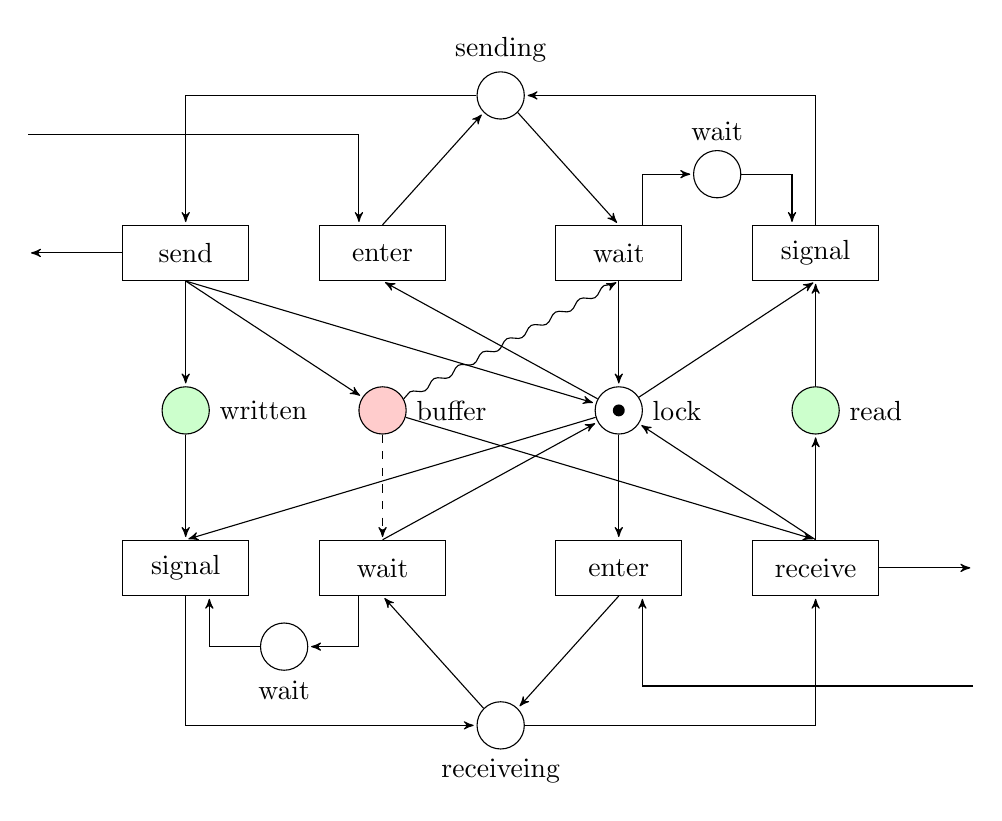
\begin{tikzpicture}
 \tikzstyle{place}=[circle, draw, minimum size=6mm]
 \tikzstyle{multiplace}=[circle, draw, minimum size=6mm, fill=red!20]
 \tikzstyle{complexplace}=[circle, draw, minimum size=6mm, fill=green!20]
 \tikzstyle{transition}=[rectangle, draw, minimum width=16mm, minimum height=7mm]
 \tikzstyle{arr}=[->, shorten >= 1pt, >= stealth']

 \node (nsendproc) at (0,4) [place] {};
 \node [above] at (nsendproc.north) {sending};

 \node (nsend) at (-4,2) [transition] {send};
 \node (nentersend) at (-1.5,2) [transition] {enter};
 \node (nwaitsend) at (1.5,2) [transition] {wait};
 \node (nsigread) at (4,2) [transition] {signal};

 \node (nsendcond) at (2.75,3) [place] {};
 \node [above] at (nsendcond.north) {wait};

 % Main places
 \node (nwrittensignal) at (-4,0) [complexplace] {};
 \node [right] at (nwrittensignal.east) {written};
 \node (nbuffer) at (-1.5,0) [multiplace] {};
 \node [right] at (nbuffer.east) {buffer};
 \node (nlock) at (1.5,0) [place, tokens=1] {};
 \node [right] at (nlock.east) {lock};
 \node (nreadsignal) at (4,0) [complexplace] {};
 \node [right] at (nreadsignal.east) {read};

 \node (nsigwritten) at (-4,-2) [transition] {signal};
 \node (nwaitreceive) at (-1.5,-2) [transition] {wait};
 \node (nenterreceive) at (1.5,-2) [transition] {enter};
 \node (nreceive) at (4,-2) [transition] {receive};

 \node (nreceivecond) at (-2.75,-3) [place] {};
 \node [below] at (nreceivecond.south) {wait};

 \node (nreceiveproc) at (0,-4) [place] {};
 \node [below] at (nreceiveproc.south) {receiveing};

 % Send transitions
 \draw [arr] (nsendproc.west) -| (nsend.north);
 \draw [arr] (nentersend.north) -- (nsendproc.south west);
 \draw [arr] (nsendproc.south east) -- (nwaitsend.north);
 \draw [arr] (nsigread.north) |- (nsendproc.east);

 % Send wait
 \draw [arr] ($ (nwaitsend.north) + (0.3,0) $) |- (nsendcond.west);
 \draw [arr] (nsendcond.east) -| ($ (nsigread.north) - (0.3,0) $);

 % Receive transitions
 \draw [arr] (nreceiveproc.east) -| (nreceive.south);
 \draw [arr] (nenterreceive.south) -- (nreceiveproc.north east);
 \draw [arr] (nreceiveproc.north west) -- (nwaitreceive.south);
 \draw [arr] (nsigwritten.south) |- (nreceiveproc.west);

 % Receive wait
 \draw [arr] ($ (nwaitreceive.south) - (0.3,0) $) |- (nreceivecond.east);
 \draw [arr] (nreceivecond.west) -| ($ (nsigwritten.south) + (0.3,0) $);

 % Signal : written
 \draw [arr] (nsend.south) -- (nwrittensignal.north);
 \draw [arr] (nwrittensignal.south) -- (nsigwritten.north);

 % Signal: read
 \draw [arr] (nreceive.north) -- (nreadsignal.south);
 \draw [arr] (nreadsignal.north) -- (nsigread.south);

 % Buffer
 \draw [arr] (nsend.south) -- (nbuffer);
 \draw [arr] (nbuffer) -- (nreceive.north);
 \draw [arr, snake=snake, segment amplitude=0.4mm] (nbuffer) -- (nwaitsend.south);
 \draw [arr, dashed] (nbuffer) -- (nwaitreceive.north);

 % Sendlock
 \draw [arr] (nsend.south) -- (nlock);
 \draw [arr] (nlock) -- (nentersend.south);
 \draw [arr] (nwaitsend.south) -- (nlock);
 \draw [arr] (nlock) -- (nsigread.south);

 % Receivelock
 \draw [arr] (nlock) -- (nsigwritten.north);
 \draw [arr] (nwaitreceive.north) -- (nlock);
 \draw [arr] (nlock) -- (nenterreceive.north);
 \draw [arr] (nreceive.north) -- (nlock);

 % Sendcall
 \draw [arr] (-6,3.5) -| ($(nentersend.north) - (0.3,0) $);
 \draw [arr] (nsend.west) -- (-6,2);

 % Receivecall
 \draw [arr] (6,-3.5) -| ($ (nenterreceive.south) + (0.3,0) $);
 \draw [arr] (nreceive.east) -- (6,-2);

\end{tikzpicture}
\caption{Petri network of the multi receiver and multi sender queue. Calls are received
         at the enter transitions and return after a successfull send or receive.
         The green places keeps many bullet as long as any target wait is active,
         but loose their bullets otherwise. The buffer node (red) can take a limited
         number of bullets (packages). The dashed arrow suppresses transition if the
         source place has any bullets. The snake arrow suppresses transition if the
         source place is not completely filled. Both special arrows do not consume bullets. }
\end{figure}

Synchronisation issues cannot be tested (as in software test) for absence, since they may only
happen in very rare cases.
Therefore an attempt to proof correctness of the approach is presented using a petri network, shown
in fig. \ref{fig:petri} as starting point. The petri net is divided into three parts,
where the top part shows a sending thread, the bottom part a receiving thread and the places
in the middle are shared among all threads. For all proofs it must be acknowledged that there
are more sending and receing threads.

Also there are a few necessary assumptions,
\begin{itemize}
 \item Correct interpretation and implementation of the POSIX functions in the operating systems
 \item Ideal hardware, e.g. no random bit flipping, no fire
 \item Reasonable software conditions, e.g. no lack of resources
\end{itemize}

The system presented should neither dead lock, nor leave the queue in an inconsistent state.
Therefore a number of questions are discussed which can cause either situation.
A complete accessibility graph would go beyond the space available in this document.

\subsection{Are sending and receiving exclusiv?}

Inconsistency through race conditions can be avoided by locks.
It must be shown, that the locks are freed upon completion and only
held by one thread at the same time.

The situation is symmetric with only one lock bullet in the initial state.
For entering either sender or receiver, the lock bullet is consumed.
From this only two transitions are possible,
\begin{itemize}
 \item Send/Receive
 \item Wait
\end{itemize}
which both give up the lock.
If a wait state is active, the signal transition can only happen if the
the lock is available. Therefore no two threads can enter sending or
receiving at the same time.

\subsection{Is it possible to be stuck in receive wait?}

Receive wait can only be entered if the buffer is empty. Any send changing this
will emit a "written" signal, which will not be lost since a receive wait state is active
and cannot be lost without the lock which is only available once the signal is emitted.

\subsection{Is it possible to be stuck in send wait?}

Send wait can only be entered if the buffer is full. Any receve changing this
will emit a "read" signal, which will not be lost since the send wait state is active.
It cannot be lost for the same reason in receive wait.

\subsection{Is it possible to be stuck in sending state?}

Either the buffer is not full, then send is available. If the buffer is full, wait is available.

\subsection{Is it possible to be stuck in receiving state?}

Either the buffer is empty, then wait is available. If the buffer is not empty, receive is possible.

\section{Measurements}
Two measurements have been made. The first being the total time $T$ required to send a number of messages.
The second being the time required for a message to arrive at any receiving thread, called $\Delta q$.
The average time required for each message is calculated by,
\begin{equation}
 s = \frac{T}{N}
\end{equation}
with N as the total number of messages send.

Still the number of possible combinations is very large with any number of sending and receiving threads
and associated loads.

Here only two very simple setups are tested,
\begin{enumerate}
 \item One sending thread, one receiving thread
 \item Two sending threads, two receiving threads
\end{enumerate}
where each sending thread sends 1 million messages without delay.
For the second measurement, only the $\Delta q$ for messages of send by the
first thread are used.

For all measurements, \texttt{CLOCK\_MONOTONIC} is used.
\FloatBarrier

Results are shown in fig.\ref{tab:resdebian}, fig.\ref{tab:resneutrino} and fig.\ref{tab:resbsd}.

\begin{table}
\label{tab:resdebian}
\centering
\begin{tabular}{l l l l}
 Setup & $T$/µs & $\Delta q$/µs & $s$/µs \\
 \hline
 1 & 3839609 & $968\pm 1356$ & 3,8 \\
 2 & 6048373 & $1451\pm 1250$ & 3,0 \\
\end{tabular}
\caption{VirtualBox 4.1.22 (4 cores assigned) running amd64 debian linux.
         Numbers behind $\pm$ are the standard deviates.}
\end{table}

\begin{table}
\label{tab:resneutrino}
\centering
\begin{tabular}{l l l l}
 Setup & $T$/µs & $\Delta q$/µs & $s$/µs \\
 \hline
 1 & 9586533 & $1797\pm 2413$ & 9,59 \\
 2 & 28430649 & $5219\pm 4508$ & 14,22 \\
\end{tabular}
\caption{VMWare Player 5.0.2 (4 core assigned) running x86 QNX Neutrino 6.5.0.
         Numbers behind $\pm$ are the standard deviates.}
\end{table}

\begin{table}
\label{tab:resbsd}
\centering
\begin{tabular}{l l l l}
 Setup & $T$ & $\Delta q$/µs & $s$/µs \\
 \hline
 1 & 7757389 & $ 95\pm 536$ & 7,76 \\
 2 & 14833631 & $ 620\pm 1988$ & 7,42 \\
\end{tabular}
\caption{FreeBSD 9.1.,
         Numbers behind $\pm$ are the standard deviates.}
\end{table}
\FloatBarrier
\newpage
\mbox{}
\pagebreak
\section{Conclusion}
The implementation should be compared to different implementations to judge its speed and latency.
This could include different signal approaches,
\begin{itemize}
 \item Sending signals only once buffers are empty or full
 \item Comparison against unbounded message buffers
 \item Using Posix message passing
 \item Using Neutrino native message passing
 \item Comparison to pipes
\end{itemize}

Also results among the different plattforms vary, and they are not well explained.
There should be a deeper analysis why there is a very short $\Delta q$ for FreeBSD 9.1.

The implementation has been tested for correctness with \texttt{testdelivery}, it therefore
should deliver the expected results.
\end{document}